% !TeX root = ../main.tex

\chapter{网格切割的基本方法}

\section{基本概念}

本文研究的网格是指由顶点,边和三角面片组成的(紧)曲面网格。形式上来说,此处定义的网格可以看作一个满足如下约束的集合 $ \mathcal M $,其中:
\begin{itemize}
  \item 集合中的元素为 0-单形(点),1-单形(直线段)或 2-单形(三角面)
  \item 集合中任意两个元素的交集仍在集合中,如两个 1-单形的交集仍在网格上
\end{itemize}

这样的网格记作 $ \mathcal{M} (V, E, F) $ ,其中 $ V $ 为顶点子集,$ E $ 为边子集,$ F $ 为面子集。

自然的,网格可以看作光滑曲面的分片近似,所以我们可以将曲面的相关概念也拓展到离散情形中。我们知道,二维流形是在每个局部与 $ \mathbb{R}^2 $ 同构的曲面,则定义任意一条边相邻的三角面片数量不超过两个的网格为流形网格。

常见的几何处理方法都需要流形网格本身是可定向的,这主要是因为无边界的二维流形无法在无自交的情形下嵌入到 $ \mathbb{R}^3 $ 中。

网格的切割,直观上说就是“沿着缝隙把曲面裁开”的过程,如图 \ref{fig:meshcut} 所示。给定一个边集合 $ \mathcal C $ 满足 $ |C| > 1 $,切割过程可以定义为一个边和网格的作用 $ \mathcal{M} \times E \to \mathcal{M'} $,其中 $ \mathcal{M'} $ 满足如下性质:
\begin{itemize}
  \item $ f = f' $ \quad (面的数量和位置保持不变)
  \item $ f \in \mathcal{M} $ 且 $ \partial f \cap C = \emptyset $,则 $ \partial f = \partial f' $  \quad (不在割缝上的边保持不变)
  \item $ f \in \mathcal{M} $ 且 $ \partial f \cap C \ne \emptyset$,则对使得 $ e_p \in \partial f_m $ 且 $ e_p \in \partial f \cap C $ 的 $ e_p $,有 $ e_p \notin \partial f' \cap f'_m $  \quad (在割缝上的边所相邻的两个三角面现在不相邻)
\end{itemize}

\begin{figure}[h]
  \centering
  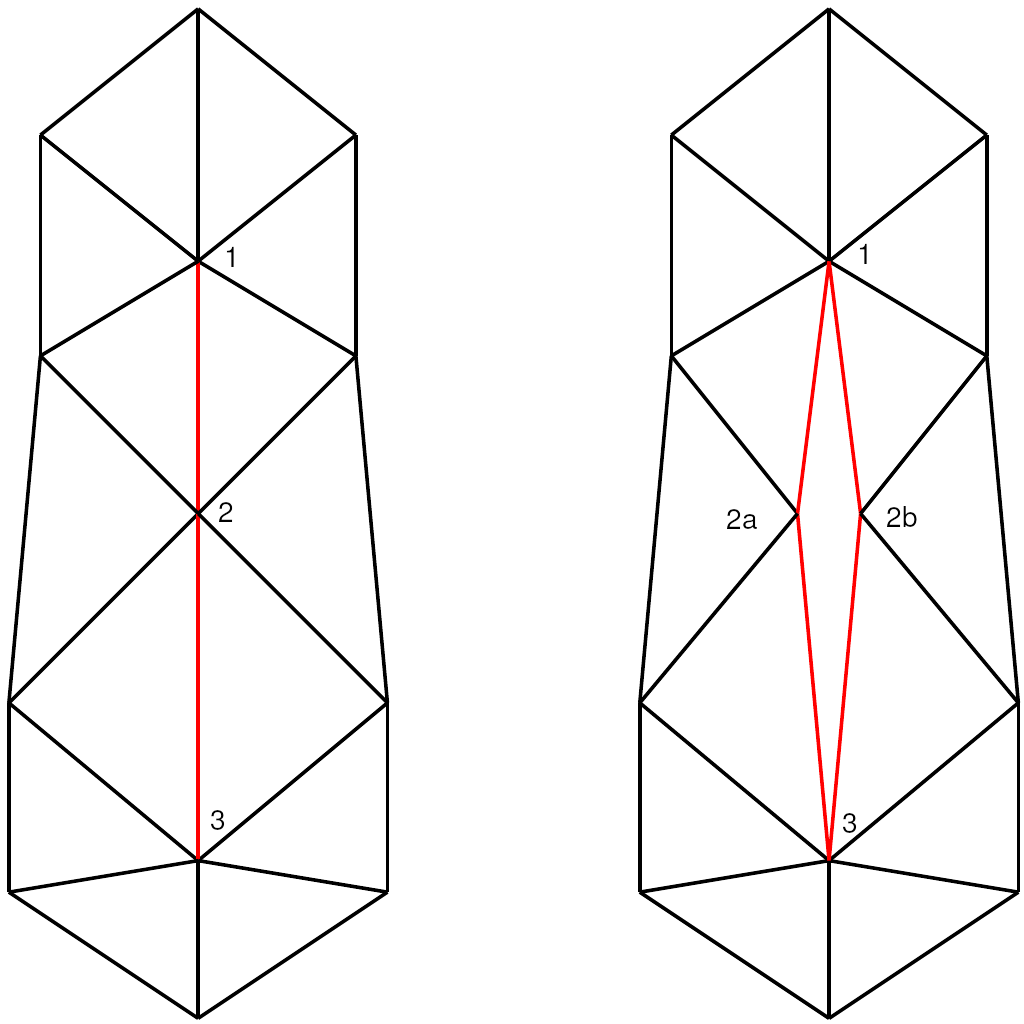
\includegraphics[width=0.5\textwidth]{tikzit_meshcut.png}
  \caption{曲面切割示意图,红色为割线}
  \label{fig:meshcut}
\end{figure}

注意到满足上述定义的过程有很多种,但是我们通常会要求切割后的网格增加的边数最少,以及切割后网格中面的几何位置不改变。

我们关心的展开成拓扑圆盘的切割,即是寻找一些特定的 $ C $ ,使得其进行切割作用后,剩余的网格构成圆盘拓扑。

\section{沿割线切割曲面}

对于已知割线集合 $ C $ 的情形,本节探讨如何从 $ C $ 得到切割后的曲面 $ \mathcal M' $。

从割线的定义出发,可以得到一个较为朴素的办法:我们可以将所有三角面分割成为一个个的孤岛,如果两三角面片相邻的边不属于割线,则将两三角面片“岛屿”相连。可以观察到,此方法的时间复杂度正比于 $ | E | + | F | $。

不过,曲面切割本质上是一个局域操作,上述操作的复杂度过高。考虑到割线作为边集合,如果加上在边上的点,就可构成无向图 $ G(V_C, C) $。此时我们可以进行如下操作:
\begin{enumerate}
  \item 对图 $ G $ 的每个连通片 $ G_i $ 的边 $ v_iv_j $, 添加 $ e' = v_i v_j $ 使得 $ v_i v_j $ 变成重复度为 2 的重边
  \item 利用 Fleury 算法计算每个 $ G_i $ 的欧拉回路 $ v_i v_j v_k ... v_i $
  \item 从起点开始遍历欧拉回路路径,设遍历到 $ v_m v_n $,令前序顶点引用 $ v_{pre} $ 初值为 $ v_i $
        \begin{itemize}
          \item 如果 $ v_n v_m $ 未遍历过,则增加新顶点 $ v'_n $。构造 $ e' = v_{pre} v’_n $ 并将 $ v_{pre} v_n $ 右侧的三角面的顶点和边分别替换为 $ v_{pre} $,$ v'_n $ 和 $ e = v_{pre}, v'_n $,同时更新 $ v_{pre} $ 引用为 $ v'_n $
          \item 如果 $ v_n v_m $ 已经遍历过,则更新 $ v_{pre} $ 引用为 $ v_m $
        \end{itemize}
\end{enumerate}

不过,上面的算法只对无边界的网格适用,对于有边界的网格,应用上面的做法可能会将流形网格切为非流形网格,如图 \ref{fig:meshboundarycase} 所示。此时,我们应该对边界点的情况进行单独处理,即在第三步遍历时,如果起点或终点的某个点为边界点,则将其完全断开。

\begin{figure}[h]
  \centering
  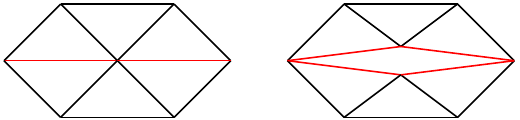
\includegraphics[width=0.6\textwidth]{tikzit_boundarycase.png}
  \caption{有边界网格情况示意,红色为割线}
  \label{fig:meshboundarycase}
\end{figure}

\section{简单网格切割算法实例}

本节以 \citet{Gu2002} 中提出的网格切割算法为例,通过实例介绍一个简单的网格切割算法是如何构造的。

\citet{Gu2002} 中提出的网格切割算法可以由一个简单的想法产生:三角面片本身是圆盘拓扑。那么,如果我们假设初始时选择一个三角面,在每次迭代时向集合 $ A $ 加入这样的三角面:他只与某个在 $ A $ 中的三角面有一条边相接,如果有更多边相接,就将剩余的边切开。

这样一来,每次迭代结束时就都是圆盘拓扑,直到 $ A $ 中有所有的三角面。对于连通的网格来说,这种方法就可以找到一个割线集合,且切割后为圆盘拓扑。

同时,我们可以观察到,割线集作为边集合构成的无向图 $ G $,可以分解成为许多圈和树边的并,而在网格内部给割线集增加树边,并不会改变切割的拓扑。这样,我们可以得到该网格切割算法的核心思想。

算法由两阶段组合而成。第一阶段时,算法不停的寻找一个不在边界上,且只与一个三角面 $ t $ 相邻的边 $ e $,并且将 $ e $ 和 $ t $ 移除。在此阶段结束时,就可以得到一个已经可以将网格切割为圆盘拓扑的割线集。第二阶段时,算法不停的寻找割线集的树边并删除,从而化简割线集。

在第一阶段,为了尽量得到“最小半径”的切割,在选择移除的三角面时可以使用种子三角面的测地线距离进行选择。

\begin{algorithm}[h]
    \SetAlgoLined
    \KwData{要切割的网格}
    \KwResult{割线集 $ C $}

    移除种子三角面\;
    \While{有只和一个三角面 $ t $ 相邻的边 $ e \notin B $} {
      移除 $ e $ 和 $ t $\;
    }
    \While{有只有一条相邻的边 $ e $ 的 $ v $ } {
      移除 $ v $ 和 $ e $\;
    }
    \caption{来自 Geometry Images \cite{Gu2002}的网格切割算法}
\end{algorithm}

% \section{计算最短割线集是 NP-Hard 问题}

% \citet{Erickson2002} 中给出了最短割线集是 NP-Hard 问题的证明。证明本身是通过将问题等价转化到已知的 NP-Hard 问题,即 \textit{直角多角形 Steiner 树问题}实现的。

% \textit{直角多角形 Steiner 树问题},即给定平面上 $ m \times m $ 正方形网格中的 n 个点,寻找最短的水平和垂直连通线段集合,使得线段集合包含所有这 n 个点。此问题即使对于 $ m $ 是 $ n $ 的多项式的情形下也是 NP-Hard 的。
